%%%%%%%%%%%%%%%%%%%%%%%%%%%%%%%%%%%%%%%%%%%%%%%%%%%%%%%%
% IE 643 Course Project poster -- Binary_Brains
% Built on the official IE643 poster template (a0poster class, portrait).
% The PDF is printed on A1: A0 and A1 have the same aspect ratio, so the page scales exactly.
%%%%%%%%%%%%%%%%%%%%%%%%%%%%%%%%%%%%%%%%%%%%%%%%%%%%%%%%
\documentclass[a0,portrait]{a0poster}
\usepackage[top=2.5cm, bottom=0.3cm, left=4cm, right=3cm]{geometry}
\usepackage[compact]{titlesec}
\usepackage{multicol}
\columnsep=70pt
\columnseprule=15pt
\raggedcolumns
\usepackage[svgnames]{xcolor}
\usepackage{palatino}
\usepackage{xkeyval}
\usepackage{graphicx}
\setlength{\abovecaptionskip}{5pt plus 5pt minus 3pt}
\graphicspath{{figures/}}
\usepackage{booktabs}
\usepackage[font=small,labelfont=bf]{caption}
\usepackage{amsfonts, amsmath, amsthm, amssymb}
\usepackage{csquotes}
\usepackage{wrapfig}
\usepackage{multirow}
\usepackage{makecell}
\def\columnseprulecolor{\color{NavyBlue}}%
\usepackage{framed}
\colorlet{frameborder}{NavyBlue}
% --- additions to the template
\usepackage{qrcode}
\usepackage{enumitem}
\setlist[itemize]{leftmargin=1.2em, itemsep=1pt, topsep=2pt, parsep=0pt}
\setlist[enumerate]{itemsep=1pt, topsep=2pt, parsep=0pt}
\captionsetup{skip=4pt}
\setlength{\abovedisplayskip}{4pt}\setlength{\belowdisplayskip}{4pt}
\setlength{\abovedisplayshortskip}{2pt}\setlength{\belowdisplayshortskip}{2pt}
\usepackage{colortbl}
\usepackage{url}
\definecolor{adj}{HTML}{2A78D6}
\definecolor{pinn}{HTML}{EB6834}
\definecolor{joint}{HTML}{14855C}
\definecolor{ink2}{HTML}{52514E}
\definecolor{band}{HTML}{EEF4FC}
\newcommand{\hl}[1]{\textbf{\color{NavyBlue}#1}}
\newcommand{\figcap}[1]{\captionof{figure}{\color{Blue}#1}}
\titlespacing*{\section}{0pt}{14pt}{6pt}

\begin{document}
\begin{minipage}[c]{\linewidth}
\vspace{0.1cm}
\noindent\makebox[\textwidth][c]{
\begin{minipage}[c]{0.14\linewidth}
\vspace{0pt}\raggedright
\hspace{1cm}

\includegraphics[width=0.8\linewidth]{figures/logo.png}
\end{minipage}
\hfill
\begin{minipage}[c]{0.75\textwidth}
\centering
\Huge \color{Green} \textbf{IE 643 Course Project}\\[0.3cm]
\LARGE \color{NavyBlue} \textbf{PINN-Based Inverse Estimation of Spatially Varying Diffusion Coefficients}\\[0.3cm]
\Large \color{NavyBlue} \textbf{Team: Binary\_Brains}\\[0.3cm]
\large \color{Black} \textbf{Jash Taparia $^{1}$ (24B2451), Mihir Gune $^{2}$ (24B2443)}\\[0.2cm]
\small \text{24b2451@iitb.ac.in$^{1}$, 24b2443@iitb.ac.in$^{2}$}\\
\end{minipage}
\begin{minipage}[c]{0.145\textwidth}
\vspace{0pt}\raggedleft

\includegraphics[width=0.8\linewidth]{figures/IE643-Logo.pdf}
\hspace{1cm}
\end{minipage}}
\\[0.1cm]%
\color{NavyBlue}\setlength\FrameRule{25pt}
\begin{framed}
\vspace{0.1cm}
\begin{multicols}{3}
\small\color{Black}
%----------------------------------------------------------------------------------------
\section*{Abstract}
We recover an unknown diffusivity map $D(x,y)$ in the 2-D heat equation from sparse, noisy sensors with a
\textcolor{pinn}{\textbf{PINN}} and a \textcolor{adj}{\textbf{Crank--Nicolson adjoint}}, on identical data. With
known physics the adjoint is $\sim2\times$ more accurate; a \textcolor{joint}{\textbf{combined}} PINN$\to$adjoint
method matches it but does not beat it. Every apparent PINN win traced to a weak time integrator or to physics the
classical method was not asked to estimate.

%----------------------------------------------------------------------------------------
\section*{Introduction}
\textbf{Problem.} From a few noisy thermometers on a plate of mixed materials, find the diffusivity everywhere:
\[
\begin{array}{ll}
\dfrac{\partial u}{\partial t} = \nabla\!\cdot\!\big(D(x,y)\,\nabla u\big) + f(x,y), & (x,y)\in[0,1]^2\\[6pt]
u(x,y,0)=u_0(x,y) & \text{initial state (two bumps)}\\
u = g(t)\ \text{on the walls} & g=0,\ f=0 \text{ (benchmark)}\\
d_k = u(x_k,y_k,t_k)+\varepsilon_k, & \varepsilon_k\sim\mathcal N(0,\sigma^2)
\end{array}
\]
\begin{center}
\renewcommand{\arraystretch}{1.25}
\begin{tabular}{p{0.22\linewidth}p{0.70\linewidth}}
\toprule
\textbf{Known} & initial state $u_0$, noise level $\sigma$; wall temperature $g$ and source $f$ (standard setting) \\
\textbf{Measured} & readings $d_k$: 5 -- 3\,969 sensors $\times$ 1 -- 200 times, 0 -- 10\,\% noise \\
\textbf{Estimated} & \hl{the full field $D(x,y)$}; in the unknown-physics setting \emph{also} the walls $g$ or the source $f$ \\
\bottomrule
\end{tabular}
\captionof{table}{\color{Blue}The inverse problem: $u$ is seen only at the sensors.}
\end{center}
\begin{itemize}
\item \textbf{Hard:} ill-posed; many $D$ fit the readings, and $D$ shows only where heat flows.
\item \textbf{Why deep learning:} a PINN needs no adjoint code, is mesh-free and enforces physics softly, so it is
claimed to tolerate imperfect physics and noise [1,4]. Relevant to thermography, drug transport, groundwater.
\end{itemize}


%----------------------------------------------------------------------------------------
\section*{Workflow}
\begin{center}
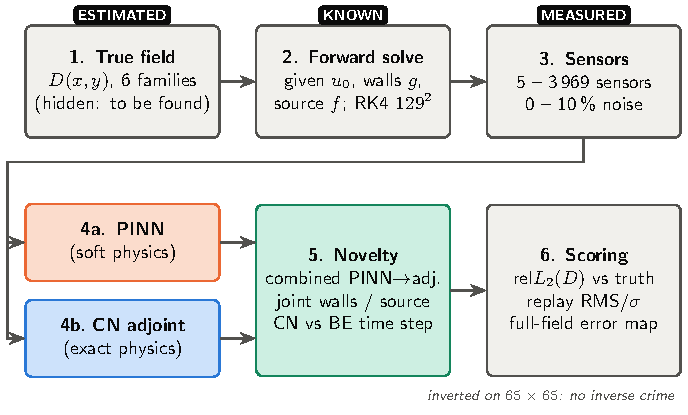
\includegraphics[width=0.90\linewidth]{F1_workflow_col.pdf}
\figcap{Workflow. Tags mark what is estimated, known and measured; both methods invert the same readings.}
\label{workflow}
\end{center}

%----------------------------------------------------------------------------------------
\section*{Methodology}
\noindent\begin{minipage}{\linewidth}
\centering
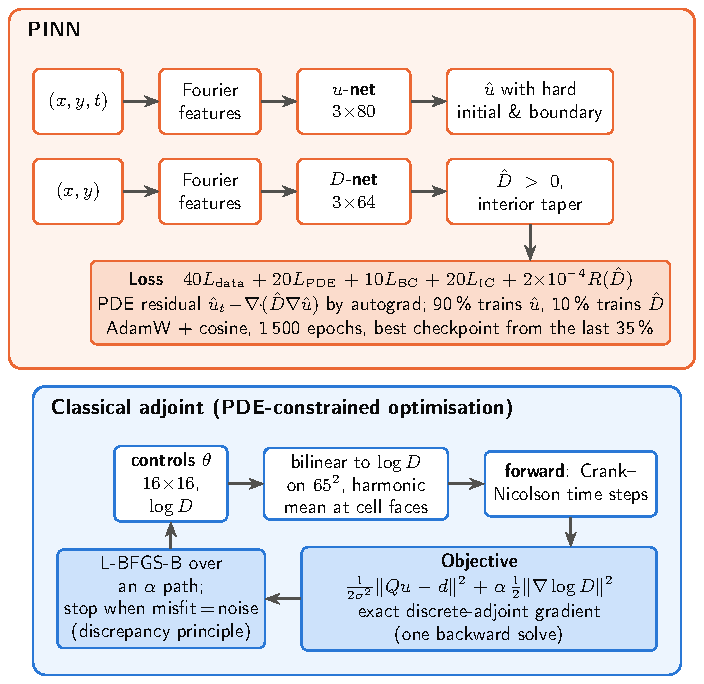
\includegraphics[width=0.78\linewidth]{F2_architecture.pdf}
\figcap{Top: PINN. Bottom: classical adjoint with a Crank--Nicolson solver.}
\label{Arch}
\end{minipage}

\begin{itemize}
\item \textcolor{adj}{\textbf{CN adjoint:}} $\log D$ on $16\times16$ controls, 100 CN steps, exact adjoint
gradient, L-BFGS-B; $\alpha$ by the discrepancy principle.
\item \textcolor{pinn}{\textbf{PINN:}} loss = data + PDE residual + initial/boundary + smoothness; AdamW, 1\,500 epochs.
\item \textcolor{joint}{\textbf{Combined:}} PINN's $\log D$ projected onto the controls starts L-BFGS-B
(also: PINN as prior, adjoint$\to$PINN). \textcolor{joint}{\textbf{Joint:}} adjoint also estimates walls or $f\ge0$.
\item \textbf{Metrics:} rel$L_2(D)=\lVert\hat D-D\rVert/\lVert D\rVert$ (needs the truth) and
\hl{replay RMS$/\sigma$}: re-simulate $\hat D$ and compare with the readings ($\approx1$ = fits to the noise level).
\end{itemize}


%----------------------------------------------------------------------------------------
\section*{Dataset Details}
\begin{center}
\renewcommand{\arraystretch}{1.2}
\begin{tabular}{ll}
\toprule
Generation & own solver, RK4, $129^2$ grid, fixed seeds \\
True $D$ & smooth, bump, inclusion, layered, random, defects \\
Datasets & 389 benchmark + 57 PINN-favoured \\
Sensors & 5 -- 3\,969: random, grid, clustered, edge \\
Readings & 1 -- 200 times per sensor \\
Noise & Gaussian, $\sigma = \eta\cdot$RMS$(u)$, $\eta = 0, 1, 5, 10\,\%$ \\
\bottomrule
\end{tabular}
\captionof{table}{\color{Blue}Dataset characteristics (synthetic, reproducible).}
\end{center}

%----------------------------------------------------------------------------------------
\section*{Novelty Assessment}
After the intensive assessment, all on the \hl{same observations, grid, source and boundary settings}:
\begin{enumerate}[leftmargin=1.4em, itemsep=4pt]
\item \textbf{PINN vs CN adjoint} on 20 datasets, 5 PINN seeds.
\item \textbf{Combined method} (4 PINN$\leftrightarrow$adjoint couplings) vs both.
\item \textbf{Unknown physics:} hidden walls (8), hidden heater (6); classical joint inversion as a rival.
\item \textbf{Controlled solver comparison:} CN vs backward Euler, with a causal test.
\item \textbf{Sensor density} 20 -- 3\,969, and 16$\times$ longer PINN training.
\end{enumerate}

\end{multicols}
\vspace{-0.6cm}
\color{NavyBlue}\noindent\rule{\linewidth}{15pt}\color{Black}
\section*{Results: the same observations, grid, source and boundary settings for every method}
\small
\noindent\begin{minipage}[t]{0.38\linewidth}
\textbf{(a) Head-to-head.} Median rel$L_2(D)$ (lower is better); replay RMS$/\sigma$ in brackets
($\approx1$ = fits the data to the noise level). Columns: known physics, hidden walls, hidden source (datasets).\\[0.3cm]
\renewcommand{\arraystretch}{1.35}
\begin{tabular}{lccc}
\toprule
 & \textbf{known (20)} & \textbf{walls (8)} & \textbf{source (6)} \\
\midrule
\textcolor{adj}{\textbf{CN adjoint}} & \textbf{0.226} (0.97) & 4.36 (15.0) & 3.29 (\hl{0.99}) \\
\textcolor{pinn}{\textbf{PINN}} & 0.468 (3.56) & 0.338 (2.48) & 0.534 (5.63) \\
\textcolor{joint}{\textbf{combined PINN$\to$adj.}} & \textbf{0.225} (0.96) & 0.296 (0.92) & 3.57 (0.99) \\
\textcolor{joint}{\textbf{joint classical}} & -- & \textbf{0.264} (0.98) & \textbf{0.169} (0.97) \\
\midrule
true-physics bound & -- & 0.201 & 0.156 \\
\bottomrule
\end{tabular}\\[0.3cm]
{\color{Blue}\footnotesize 5 seeds: PINN 0.468 -- 0.554, combined 0.223 -- 0.228; PINN beats CN adjoint in 3/100
dataset--seed pairs. Walls ``combined'' = joint inversion started from the PINN's walls.}
\end{minipage}\hfill
\begin{minipage}[t]{0.58\linewidth}
\textbf{Reading the table.}
\begin{itemize}
\item \textbf{Known physics:} the CN adjoint is $\sim2\times$ more accurate and fits the data to the noise level;
the PINN does not ($3.6\sigma$). The combined method returns the adjoint's answer.
\item \textbf{Hidden walls or source:} an adjoint enforcing the wrong PDE must bend $D$, so the soft-physics PINN
wins --- until the classical method estimates the missing term jointly with $D$: then it wins on 7/8 and 6/6
datasets, near the true-physics bound.
\item \textbf{Replay can mislead:} with the hidden source the adjoint fits the sensors to $0.99\sigma$ yet its $D$ is
wrong everywhere (rel$L_2$ 3.29). A good sensor fit does not prove the field is recovered, so we always show
the full field and its error map (b).
\item \textbf{Sensor density} barely helps the PINN (0.481 $\to$ 0.404 from 20 to 3\,969 sensors) but helps the
adjoint (0.156 $\to$ 0.070); 16$\times$ longer training takes the PINN from 0.384 to 0.132: its limit is training.
\end{itemize}
\end{minipage}

\vspace{0.2cm}
\textbf{(b) True vs recovered full fields, spatial error maps and replay} (same 50 sensors, white dots, for every method).
\begin{center}
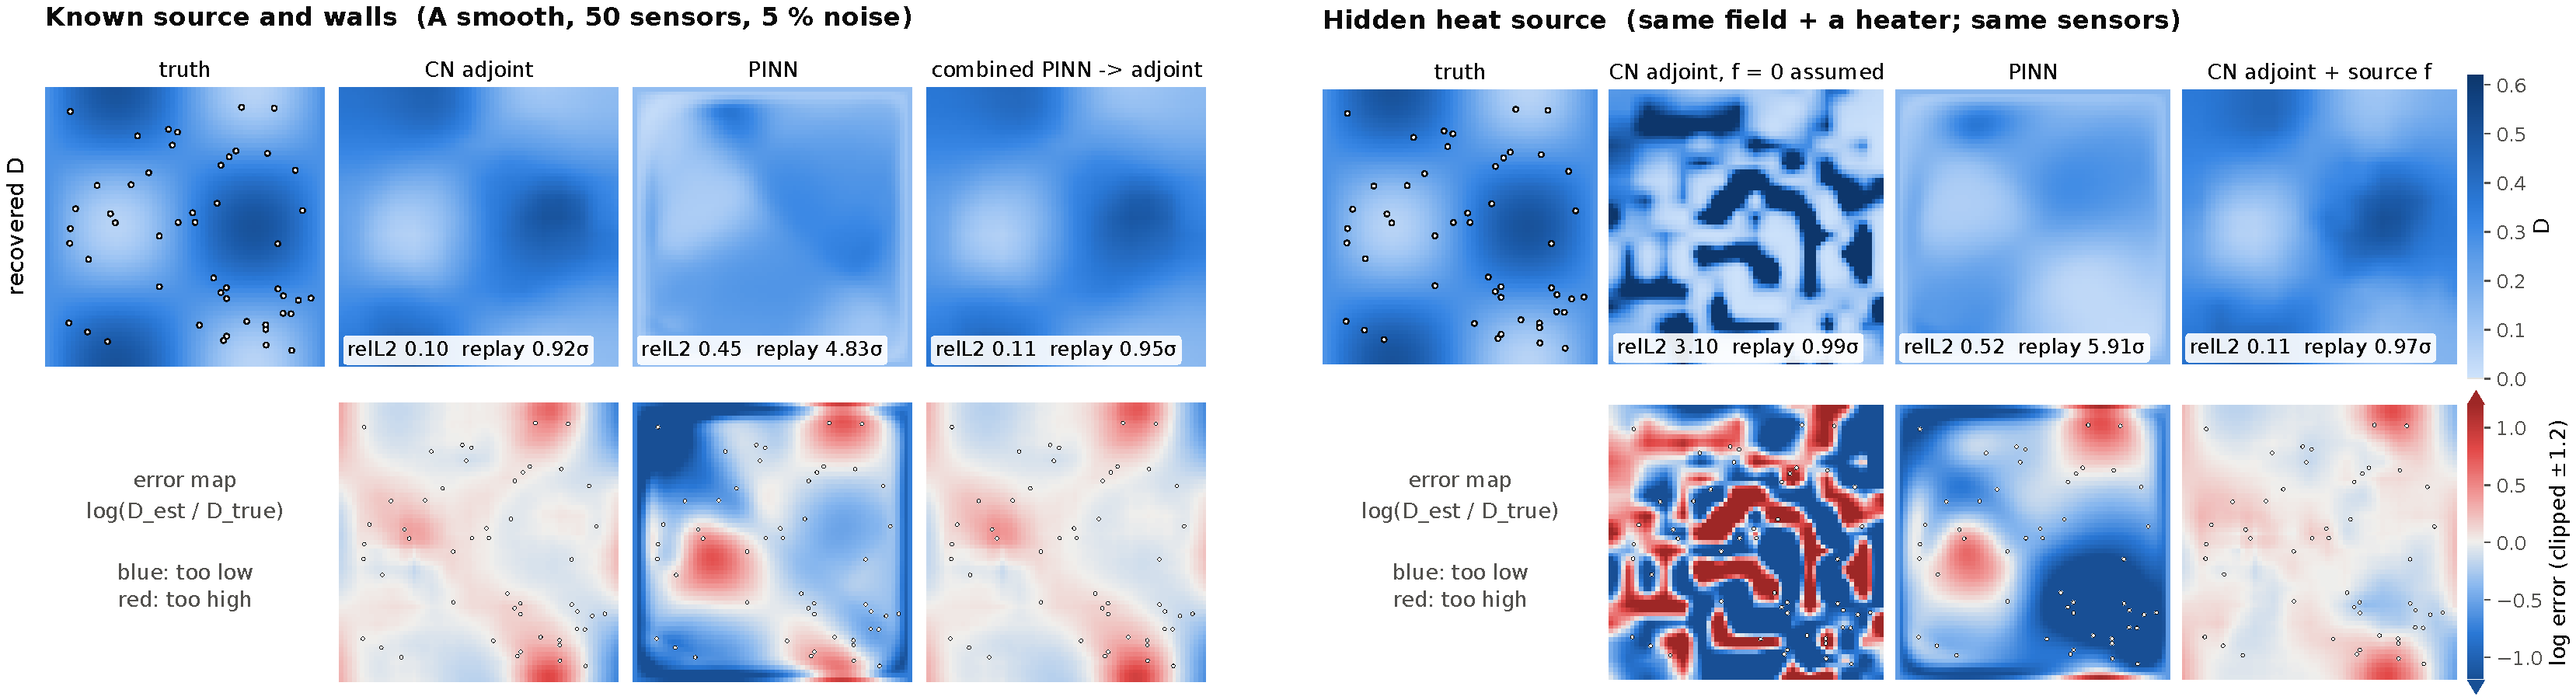
\includegraphics[width=0.78\linewidth]{F12_fields_errors_replay.pdf}
\figcap{Left: the CN adjoint and the combined method recover the structure; the PINN's field is flattened and too low
at the walls. Right: assuming no source, the adjoint fits the readings ($0.99\sigma$) with a wrong $D$; estimating the source fixes it.}
\end{center}
\color{NavyBlue}\noindent\rule{\linewidth}{15pt}\color{Black}
\vspace{-0.4cm}
\begin{multicols}{3}
\small
\section*{Results: does the solver decide?}
\textbf{(c) Controlled solver comparison.} The intensive-phase ``PINN wins with dense sensors'' used a backward-Euler
(BE) adjoint. Same adjoint and data; only the integrator changes:
\begin{center}
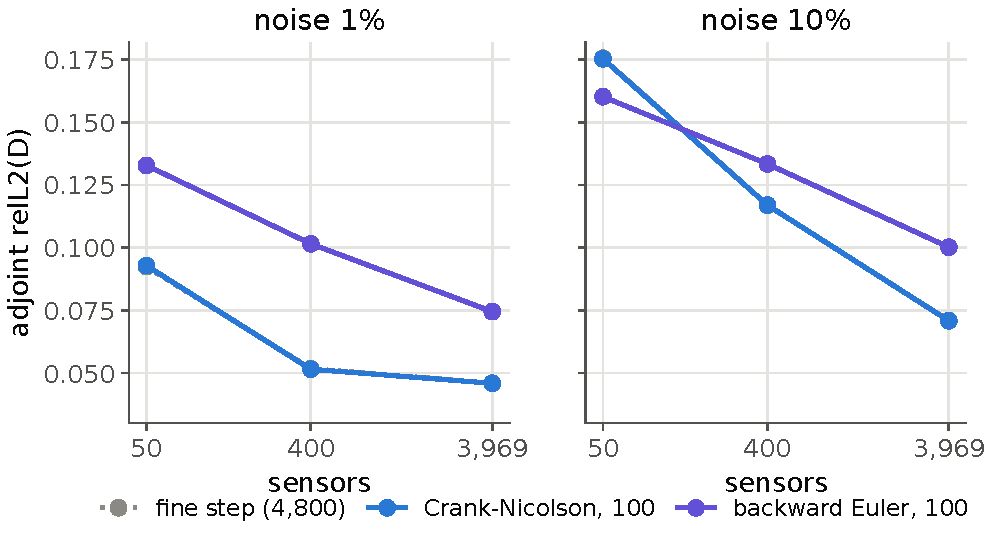
\includegraphics[width=0.95\linewidth]{F10_time_integrator.pdf}
\figcap{CN with 100 steps lies on the 4\,800-step reference; BE is worse in 8 of 9 noise/density cells (3\,969
sensors, 1\,\%: 0.074 vs 0.046), least so at high noise. On the same data the PINN reaches 0.384 (0.132 after
16$\times$ longer training).}
\end{center}
\begin{itemize}
\item \textbf{Why:} BE decays too slowly ($1/(1+x)$ vs $e^{-x}$), acting like a smaller $D$; its temperature error
is only 2.9\,\% of the signal but \hl{2.5$\sigma$ at 1\,\% noise}, so the inversion inflates $D$ and invents structure.
\item \textbf{Causal test:} on data generated by BE itself, BE inverts as well as CN (0.093/0.093, 0.053/0.051,
0.047/0.046). The solver must be accurate \emph{relative to the noise}; the PINN's win was this artefact.
\end{itemize}





%----------------------------------------------------------------------------------------
\section*{Conclusion}
\begin{itemize}
\item On matched data with known physics the \textcolor{adj}{\textbf{CN adjoint}} is about $2\times$ more accurate
than the PINN and fits the data to the noise level; the PINN does not (replay $3.6\sigma$).
\item The \textcolor{joint}{\textbf{combined method}} matches the adjoint, not more: the strongly regularised start of the
$\alpha$ path pulls any start to the same field (same final $\alpha$ on 20/20), at $\sim3\times$ the cost.
\item Replay alone can mislead: always check the full field and its error map.
\item All three apparent PINN wins were explained: a backward-Euler solver error above the noise, unestimated walls,
an unestimated source.
\item \textbf{Future work:} uncertain initial states, 3-D and real thermography data, PINNs for unknown operators
rather than coefficients, cheaper PINN warm starts for expensive (3-D) adjoints.
\end{itemize}

%----------------------------------------------------------------------------------------
\section*{References}
\footnotesize
\begin{enumerate}[label={[\arabic*]}, leftmargin=1.8em, itemsep=3pt]
\item Maziar Raissi, Paris Perdikaris and George Em Karniadakis. Physics-informed neural networks: A deep learning
framework for solving forward and inverse problems involving nonlinear partial differential equations, Journal of
Computational Physics, 2019. \url{https://doi.org/10.1016/j.jcp.2018.10.045}
\item Zhen Zhang, Alessandro Alla and George Em Karniadakis. Adjoint Method versus Physics-Informed Neural Networks
in PDE-Constrained Inverse Problems, arXiv preprint, 2026. \url{https://arxiv.org/abs/2606.12337}
\item Aleksandra Jekic, Afroditi Natsaridou, Signe Riemer-S{\o}rensen, Helge Langseth and Odd Erik Gundersen.
Examining the robustness of Physics-Informed Neural Networks to noise for Inverse Problems, arXiv preprint, 2025.
\url{https://arxiv.org/abs/2509.20191}
\item Sukirt Thakur, Ehsan Esmaili, Sarah Libring, Luis Solorio and Arezoo M. Ardekani. Inverse resolution of
spatially varying diffusion coefficient using physics-informed neural networks, Physics of Fluids, 2024.
\url{https://doi.org/10.1063/5.0207453}
\item Tamara G. Grossmann, Urszula Julia Komorowska, Jonas Latz and Carola-Bibiane Sch{\"o}nlieb. Can
physics-informed neural networks beat the finite element method?, IMA Journal of Applied Mathematics, 2024.
\url{https://doi.org/10.1093/imamat/hxae011}
\item Petr Karnakov, Sergey Litvinov and Petros Koumoutsakos. Solving inverse problems in physics by optimizing a
discrete loss: Fast and accurate learning without neural networks, PNAS Nexus, 2024.
\url{https://doi.org/10.1093/pnasnexus/pgae005}
\end{enumerate}
\normalsize

%----------------------------------------------------------------------------------------
\section*{Acknowledgments}
\small \textnormal{We thank the \textbf{IE 643 instructor and teaching assistants} for their guidance and for the
feedback from the intensive assessment.}
\normalsize

\section*{Github Link and Demo Video Link}
\vspace{-0.5cm}
\begin{center}
\begin{minipage}{0.4\linewidth}
\centering
\textbf{Github Repository}\\[1ex]
\qrcode[height=0.5\linewidth]{https://github.com/bloodrepaer/IE643-Binary-Brains-PINN-Inversion}
\end{minipage}\hfill
\begin{minipage}{0.4\linewidth}
\centering
\textbf{Demo Video Link}\\[1ex]
\fbox{\parbox[c][0.5\linewidth][c]{0.5\linewidth}{\centering\small demo-video\\QR code}}
\end{minipage}
\end{center}

\end{multicols}
\vspace{0.1cm}
\end{framed}
\end{minipage}
\end{document}
